\chapter{组件-事件知识图谱构建}
本章主要介绍了组件-事件知识图谱的构建流程。目前已有的分布式集群运行状态监测模型都不能涵盖所有种类的信息。文献\parencite{wang2019grano}只构建了组件拓扑图而忽略了组件上数据之间的因果关系;文献\parencite{nie2016mining-causality-graph}将运行时信息转为事件数据后,只关注了事件间的因果图而忽略事件所在组件之间的拓扑关系;文献\parencite{qiu2020causality-mining-knowledge-graph}尝试构建运维知识图谱,但所构建的知识图谱只包含组件间的访问与部署关系、指标与组件间的来源产生关系,对于异常信息间的触发关系,只能精确到指标时序类型之间的因果关系,如“Container
1 CPU usage”导致了“Microservice 1 Response Time”,不能进一步确定是什么样的 CPU 变化
导致了什么样的响应时间变化。本文在构建组件-事件知识图谱时,首先通过公开API(Application Programming Interface)、调用链追踪系统获取组件唯一标识符、属性和关联关系等信息;其次将日志、指标时序数据等运行时信息转为了事件类型数据,然后设计了共计6种事件特征用于发掘事件间因果关系;最后将同故障类型的组件-事件拓扑图整合起来,自动沉淀出了标有对应故障类型的组件-事件知识图谱。本章分别介绍了组件拓扑关系获取方式,事件因果关系获取方式和组件-事件知识图谱生成方式。

% 对于组件部分数据,云服务商会提供开放的API返回分布式集群含有的组件属性信息、每类组件数量及每个组件间的关联关系。在事件层面,包含着分布式应用部署、模拟触发故障、数据收集、数据清洗、事件生成、事件因果关系挖掘及事件知识图谱构建。最后根据事件来源的组件类型,即可合并组件事件数据,构建生成组件-事件知识图谱。
\section{组件拓扑关系获取}
% https://help.aliyun.com/document_detail/86742.html
\begin{figure}[htbp]
    \centering
    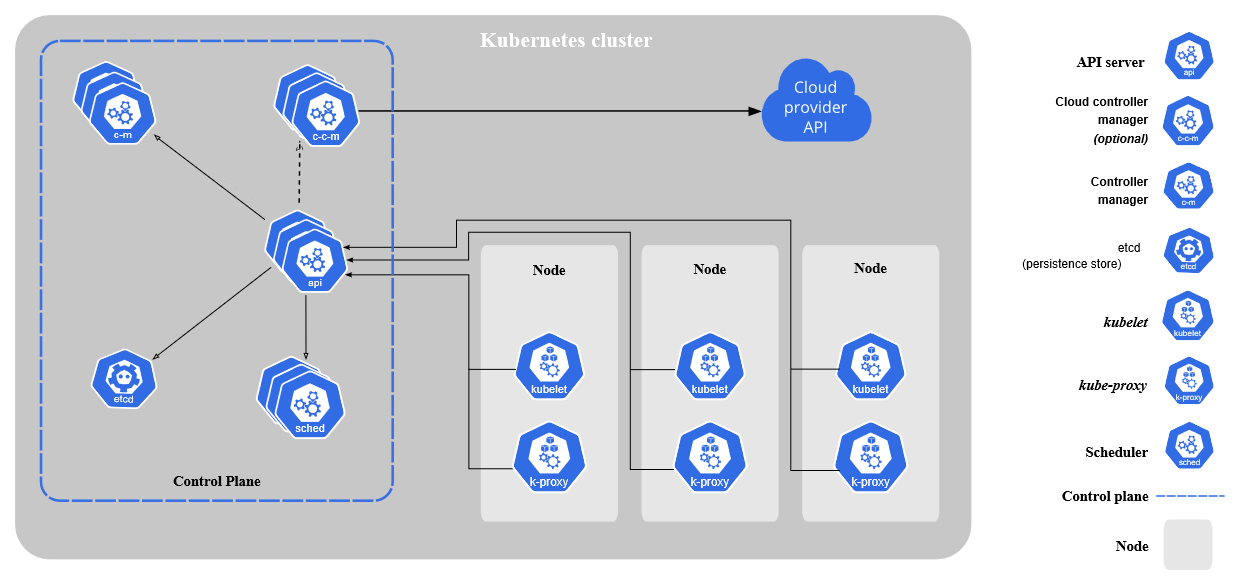
\includegraphics[width=.8\textwidth]{Kubernetes-components.png}
    \caption{Kubernetes集群结构示意图\label{Kubernetes-components}}
\end{figure}
Kubernetes集群\cite{bernstein2014containers}在云计算行业中已经被广泛使用,它是一个具有扩展性、移植性的开源平台,同时具有着清晰的声明式配置和自动化特性,被用于管理各种容器化工作负载和服务。Kubernetes集群由一组工作机器(称为节点)组成,这些节点上运行着微服务,但为微服务并不是直接运行在这些节点上,而是由节点中承载的Pod来负载这些微服务。在生产环境中,集群通常运行着多个节点,从而提供容错性和高可用性。图\ref{Kubernetes-components}为一个Kubernetes集群示意图,可见所有组件都被绑定在一起,其间存在着复杂的负载、交互等关系。

本文所使用的Kubernetes集群是阿里云针对企业级应用所优化的容器服务版Kubernetes集群,其管理容器化应用的能力具有伸缩性,性能较高。阿里云对其提供的Kubernetes集群中各类组件都进行了清晰定义,具体上各类组件类型及含义如表\ref{systemCompotent}所示。

\newcommand{\tabincell}[2]{\begin{tabular}{@{}#1@{}}#2\end{tabular}}  
\begin{table}[htbp]
    \centering
    \caption{集群组件信息}
    \begin{tabular}{cc}
    \toprule
        
        组件名称 & 含义 \\ \midrule
        VPC & \tabincell{l}{专有网络(Virtual Private Cloud,VPC)是自定义私有网络。不同的专有网络之间\\存在二层逻辑隔离。用户可以在自己创建的专有网络内创建和管理各个云产品实\\例,比如ECS、SLB 、RDS 等。}  \\
        \midrule
        SLB & \tabincell{l}{负载均衡器(Server Load Balancer,SLB)是负责对多台应用实例进行流量分发\\的负载均衡服务。用户可以通过分流提高系统的服务能力,也可以通过消除单点\\故障使其具有可用性。} \\ 
        \midrule
        ECS & \tabincell{l}{云服务器(Elastic Compute Service,ECS)是一种简单高效、具有弹性处理能力\\的计算服务。云服务器可以辅助用户高效率构建安全性、稳定性高的应用。} \\ 
        \midrule
        Pod & \tabincell{l}{Pod 是 Kubernetes 中最小的部署单元和计费单位,根据应用场景,可以由一个或\\多个容器组成。当一个 Pod 中有多个容器时,这些容器会共享 Pod 的计算资源、\\存储空间、IP和端口。对于计算资源,Pod还可以限制各个容器使用的比例。} \\ 
        \midrule
        Container & \tabincell{l}{Container即为容器,它包含在Pod中。一个Pod中有一个Pause容器和若干\\个业务容器。} \\ 
        \midrule
        Service & \tabincell{l}{微服务是一种云原生架构方法,其中单个应用程序由许多松散耦合且可独立\\部署的较小Service组成。} \\ 
    
    \bottomrule
    \end{tabular}
    \label{systemCompotent}
\end{table}

为了获取处于运行状态的Kubernetes集群中各个组件实例的唯一标识、属性和其间的关联关系,本文使用了云服务商提供的公开API进行数据的请求,如获取某区域ECS信息的API为DescribeInstances(.)方法接口,输入地理区域“cn-hangzhou”,就会返回该区域的ECS信息。图\ref{api_ecs_info}为返回的杭州区域的一台ECS的信息列表,包含该ECS的资源组、内存、唯一标识符、创建事件等属性信息,以及所属VPC的Id信息。除了Service类型组件,其它集群组件均可通过API获取其属性信息及与其他组件的关联信息。

Service类型组件对应着部署在Kubernetes集群中的分布式应用的各个微服务。微服务之间的拓扑关系与开发人员编写的应用架构结构有关,无法通过云服务商提供的公开API直接获取。分布式应用代码是其所属公司的保密性数据,不能被外部获取或改写,所以通过侵入代码获取微服务结构的方法是不可行的。目前开放式的微服务追踪系统(如Jaeger\cite{mengistu2020distributed}),可以跟踪微服务之间的请求数据,然后分析汇总这些请求链路就可以构建出微服务之间的访问拓扑关系。追踪请求数据生成微服务拓扑关系的方法不必侵入代码,也不需要运维人员阅读分布式应用的开发文档,只需要将追踪系统部署在分布式应用所在的集群中跟踪分布式应用即可。因此,本文通过云服务商提高的公开API和分布式请求跟踪系统,获取了组件部分的拓扑结构及实体属性。
\begin{figure}[htbp]
    \centering
    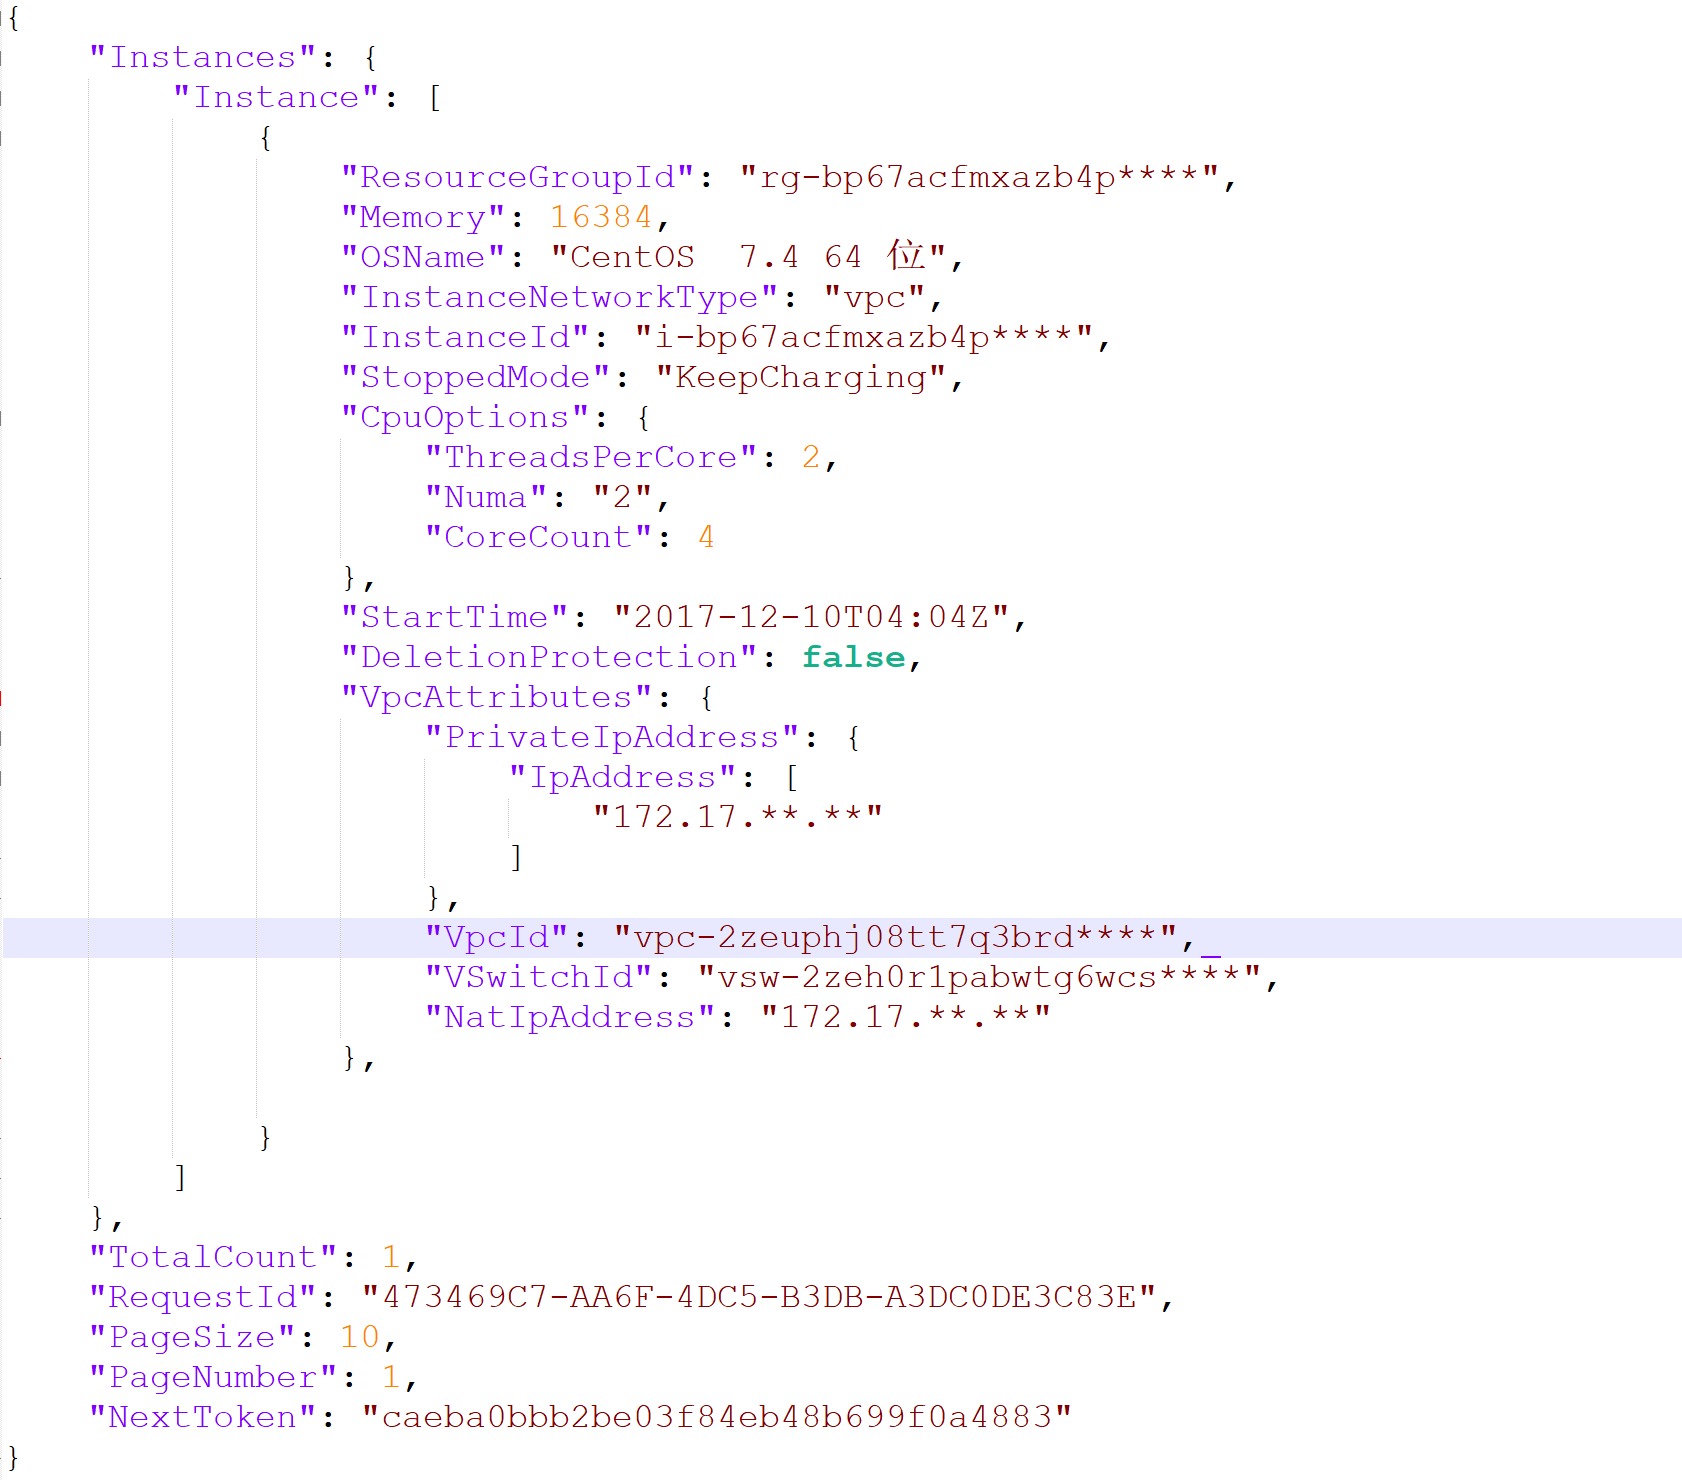
\includegraphics[width=.75\textwidth]{api_ecs_info.png}
    \caption{阿里云公开API返回ECS数据部分示例\label{api_ecs_info}}
\end{figure}

\section{事件因果关系获取}
本小结旨在将集群运行状态数据经过清洗整理后转为事件信息,并进一步经过关系分类器挖掘事件间因果关系。在事件生成部分,使用了聚类、异常识别、模板匹配结合的方式,将实时产生的日志、指标时序数据转为了事件类数据。在事件因果关系挖掘部分,为了克服过往工作中只存在基于概率的事件特征,导致领域专家需要反复标注海量数据训练模型才能达到良好效果的问题,本文设计了6种事件特征,最终不需要反复标注海量数据就可以达到优质的效果。
\subsection{事件生成}
\begin{definition}[事件]
    \label{event-define}
    事件。事件是对分布式系统中组件运行状态的描述。主要包括五个部分:
    {\\\qquad
        Id:事件的唯一标识;\\
        Time:事件发生的时间戳;\\\qquad
        Location:事件发生所在的具体组件;\\\qquad
        EventType:事件类型描述;\\\qquad
        Detail:事件的具体描述\\\qquad
    }
\end{definition}

\begin{definition}[完全周期性事件]
    \label{periodic-event}
    完全周期性事件是严格按照一定时间间隔出现的事件,如每隔3s必然出现一次。
\end{definition}

\begin{figure}[htbp]
    \centering
    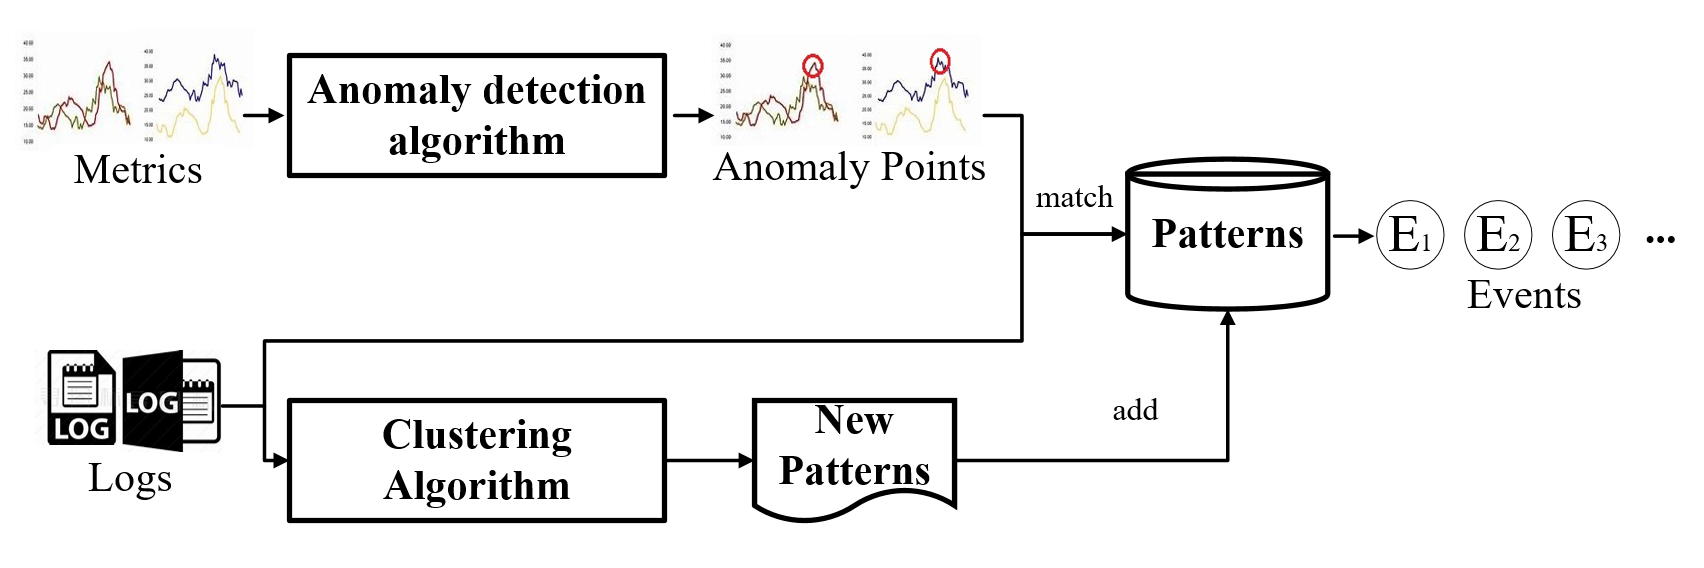
\includegraphics[width=.8\textwidth]{event-generate.png}
    \caption{事件生成流程\label{event-generate}}
\end{figure}

事件定义如Definition \ref{event-define}所示。在生成事件之前,需要先收集到指标时序数据、日志数据,本文部署了云计算相关工作常用的两个开源应用train-ticket\cite{zhou2018poster} 、sock-shop\cite{rahman2019predicting}于阿里云平台上,随后分别多次模拟了常见的故障,并收集了两个应用正常数据以及各个故障场景的异常数据。具体数据收集情况会在实验部分详细描述。

在收集完相关原始数据后,事件生成模块的主要功能是将系统的异常信息转为统一规范的事件数据,整体流程如图\ref{event-generate}所示。系统中的数据主要有两种,一种是指标时序数据,记录着系统各个组件的状态曲线变换,如内存、读写、CPU等随时间的变化曲线;另一种是日志数据,记录着微服务在具体时间戳打印的日志内容,如在某个时间微服务打印“xxx service strats success”日志。对于指标时序数据,本文首先使用异常检测算法检测到异常点,比如某些指标开始很平滑,然后经过某个点后开始抖动,那么这个转折点就是异常点,异常点一般是系统发生异常的一种表现。在找到异常点后,经过模板匹配就可以得到异常事件。比如某Container的CPU使用率曲线突然上升到100\%,那么根据模板可以得到这个异常点事件类型是“container.cpu.usage.seconds.total”。对于日志数据,一方面会使用聚类算法发掘日志中的通用模板,如果有新模板产生,那么就会添加到模板库中;另一方面会使用模板库中的模板来匹配日志生成相应事件。图\ref{log-example}中是一些日志数据,这些日志由于格式比较类似,相同的关键词也比较多,因此会被聚类算法分为一类,这一类的模板就会写为 “****-**-** **:**:**, pod *** occurs Back-off restarting failed”,随后这个模板会被添加到模板库中,之后产生的日志匹配到此类模板会生成相应的事件。上文提到的异常检测算法\cite{yang2019integrated}和聚类算法\cite{landauer2020system}目前业界已有很多,不是本文主要研究内容,所以这里就不展开对这方面的细致介绍。

\begin{figure}[htbp]
    \centering
    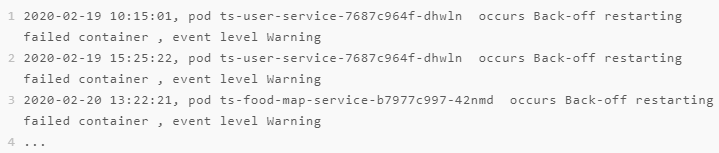
\includegraphics[width=.8\textwidth]{log-example.png}
    \caption{日志数据样例\label{log-example}}
\end{figure}

本文生成的事件按照严重等级可以划分如表\ref{event-type}所示,包括正常事件、异常事件和故障事件。正常事件是指系统内组件在正常业务逻辑中产生的事件,注意正常事件也有可能引发故障,比如事件“服务器正在重启”,虽然此事件是服务器正常重启产生的事件,但是如果在此服务器重启时,其他服务器对其访问,也会产生“访问失败”事件,触发系统故障。异常事件是指系统组件发生了正常执行业务时不会出现的事件,如异常检测算法检测到的系统异于常态的事件,但异常事件发生时组件仍可工作,不会发生系统不可用。故障事件是描述组件故障的事件,故障事件发生时系统部分服务已无法正常工作。
% Please add the following required packages to your document preamble:
% \usepackage{multirow}
% Please add the following required packages to your document preamble:
% \usepackage{multirow}
\begin{table}[htbp]
    \centering
    \caption{事件严重程度划分结果}
    \label{event-type}
    \begin{tabular}{ccc}
    \toprule
    初级划分                  & 次级划分   & 示例                                                                                                       \\ 
    \midrule
    \multirow{2}{*}{正常事件} & 硬件正常事件 & container memory 50\%、container cpu 50\%、...                                                             \\
                          & 软件正常事件 & 数据库连接成功、...                                                                                              \\ 
                          \midrule
    \multirow{2}{*}{异常事件} & 硬件异常事件 & container memory 100\%、container cpu 100\%、...                                                           \\
                          & 软件异常事件 & 数据库连接失败、...                                                                                              \\ 
                          \midrule
    \multirow{2}{*}{故障事件} & 硬件故障事件 & 服务器宕机、...                                                                                                \\
                          & 软件故障事件 & \begin{tabular}[c]{@{}c@{}}HttpServerErrorException 503、\\ HttpServerErrorException 500、...\end{tabular} \\ 
                          \bottomrule
    \end{tabular}
\end{table}

% \begin{table}[]
%     \caption{事件严重程度划分}
%     \label{event-type}
%     \begin{tabular}{llll}
%     \hline
%     事件 & 正常事件 & 硬件正常事件 & container memory 50\%、container cpu 50\%、...                  \\
%        &      & 软件正常事件 & 数据库连接成功、...                                                   \\ \cline{2-4} 
%        & 异常事件 & 硬件异常事件 & container memory 100\%、container cpu 100\%、...                \\
%        &      & 软件异常事件 & 数据库连接失败、...                                                   \\ \cline{2-4} 
%        & 故障事件 & 硬件故障事件 & 服务器宕机、...                                                     \\
%        &      & 软件故障事件 & HttpServerErrorException 503、HttpServerErrorException 500、... \\ \hline
%     \end{tabular}
% \end{table}

此外,在生成的事件中存在大量的完全周期性事件,其定义如Definition \ref{periodic-event}所示。完全周期性事件的存在,一方面使得事件数量级抖升而增加了时空复杂度,一方面会干扰后续事件因果分析、故障预测的效果。完全周期性事件不管集群有无异常都会保持绝对的周期出现,与集群状态无关。因此,在生成事件后,需要初步筛选去除具有完全周期性的事件,本文使用DTW(Dynamic Time Warping)算法\cite{mueen2016extracting}判断事件是否为完全周期性事件。采用DTW算法的原因在于该算法已经在语音匹配任务中取得了优秀的效果,它不需要曲线精确的对位分析,能适应时间错位性。利用该算法进行去除完全周期性噪声事件的具体做法为:

(1)统计某类事件$e$在异常注入前$t_1$时间段、异常到故障产生时间段$t_2$和故障发生后$t_{3}$时间段这三段时间内,发生的频次曲线。其中$t_1 = t_2 = t_3$。

(2)对比三段时间$t_1$、$t_2$和$t_{3}$所对应的三条频次曲线。如果DTW算法判别三者等同,则认为该类事件是完全周期性事件。

(3)对异常注入到故障产生时间段内的所有事件均采取上述判别过程。最终将认定有完全周期性的事件删除,只保留非完全周期性事件。该过程可以删去总事件量中约15\%的完全周期性事件,如在总共收集到的3738条事件中,删去了537条完全周期性事件。
% \begin{figure}[htbp]
%     \centering
%     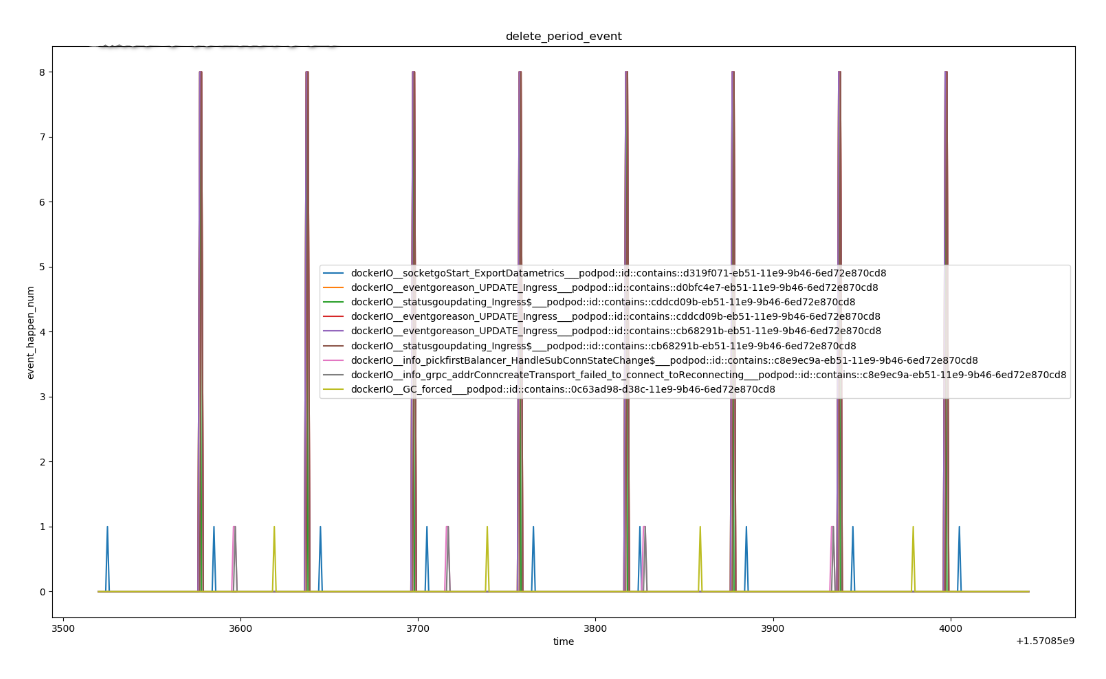
\includegraphics[width=.65\textwidth]{deleted-period-events.png}
%     \caption{筛去的完全周期性事件频次图\label{deleted-period-events}}
% \end{figure}

% 图\ref{saved-no-period-events}为保留的非完全周期性事件频次图。图\ref{deleted-period-events}为筛去的完全周期性事件频次图。可见被删去的完全周期性事件,均为集群管理系统发生的事件,如socket信息、垃圾回收信息和周期性更新信息等。

% \begin{figure}[htbp]
%     \centering
%     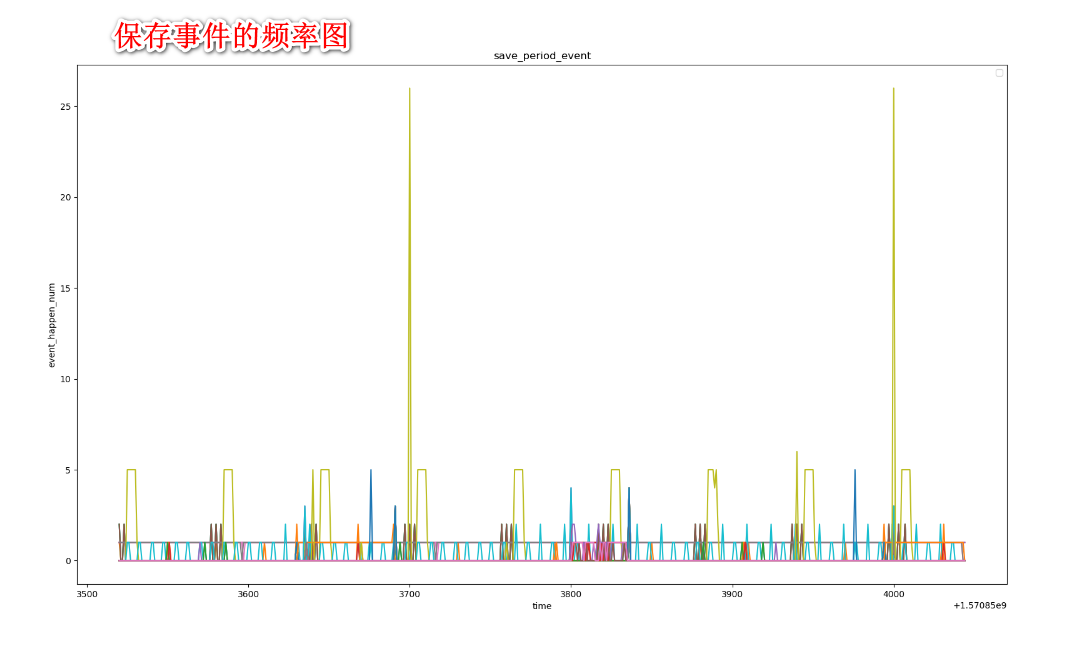
\includegraphics[width=.65\textwidth]{saved-no-period-events.png}
%     \caption{保留的非完全周期性事件频次图\label{saved-no-period-events}}
% \end{figure}
% \newpage
\subsection{事件因果关系挖掘}
关系分类器用于判别事件间关系类型,本文中为有无因果关系。输入关系分类器的是A、B两事件特征向量,输出为A到B是否有因果关系,即A→B是否存在。若要判断有无B到A(即B→A)的因果关系,需要按照顺序输入B、A两事件特征向量。本文共设计了以下6种事件特征:

(1) 皮尔逊相关系数:该特征用来计算两个事件之间的相关性,即两个事件之间的皮尔逊相关系数越高,那么这两个事件越相关,越有可能是因果关系。皮尔逊相关系数计算方法如公式\ref{1per}所示。其中$X,Y$是事件$A,B$分别在时间维度上展开的向量。当事件发生时为1,未发生时为0,事件按照在每个时间戳是否发生,可以表示为0、1组成的数字向量。
\begin{equation}
    p_{x, y}=\frac{\sum(X-\bar{X})(Y-\bar{Y})}{\sqrt{\sum(X-\bar{X})^{2}(Y-\bar{Y})^{2}}}\label{1per}
\end{equation}

(2)关系置信度:该特征用来统计历史数据中,$A$事件出现后$B$出现的概率。若$A$出现后$B$出现,则计$AB$共同出现一次。计算方式如公式\ref{2confident}所示。
\begin{equation}
    \operatorname{{ relevant }\_{confidence }}(A, B)=P(B/A)=P(\operatorname{count}(A B) / \operatorname{count}(A))\label{2confident}
\end{equation}

(3)事件发生所在设备的距离度量:根据异常沿着组件拓扑传播的特性,两事件发生所在组件位置越近,越可能是因果关系。计算方式如公式\ref{3distance}所示。其中$device(.)$为找到事件所在设备,$Distance(.)$输出两设备距离,$log(1+.)$是为了让取值均大于0。
\begin{equation}
    d(A, B)=\log (1+\text { Distance }(\text { device }(A), \operatorname{device}(B)))\label{3distance}
\end{equation}

(4)平均时间差:事件发生时间越近,越可能是因果关系。计算事件$A$和事件$B$时间差时,$A,B$均可能出现多次,这时需要计算事件$A$与$B$的平均时间差。具体计算方式如公式\ref{4timeinter}所示:统计$A$出现的时间戳序列$A_{stamps}$,统计$B$出现的时间戳序列$B_{stamps}$。统计每当$A$出现后$B$出现的时间差序列$intervals$。最终求均值$mean(intervals)$再将取值调整为均大于0,即可得到$A,B$间平均时间差。
\begin{equation}
    \operatorname{\text{time}\_{interval}}\left ( A,B \right ) =  \log\left ({1+  \operatorname{mean} \left ( B_\text{stamps} - A_\text{stamps} \right ) } \right )\label{4timeinter}
\end{equation}

(5)事件周期性度量:虽然在事件生成后,本文已经初筛去掉了完全周期性事件,但仍保留了周期性不完美的事件,如每隔4s左右会出现大约2次。由于周期性事件在故障场景与正常场景中都会以一定的周期性出现,所以具有周期性的事件一般不会引发故障。可见事件周期性越高,它与其他事件的因果关系越弱。计算方式如公式\ref{5eventspan}所示:统计事件$A$出现的时间戳序列$A_{stamps}$,随后对事件戳序列差分求标准差即可。计算结果值越小,则事件周期性越强。将$A,B$两事件周期性值较小值输入分类器即可。其中$diff(.)$表示求差分,$std(.)$表示求标准差。
\begin{equation}
    \operatorname{period}(A)=\log \left(1+\operatorname{std}\left(\operatorname{diff}\left(A_{stamps}\right)\right)\right)\label{5eventspan}
\end{equation}

(6)事件关键性度量:如果事件常发生在故障时间段内,在系统正常时很少发生,这意味着此事件很可能与故障有关并且是关键事件;反之,更可能为白噪声事件。事件关键性值可以用于衡量事件关键性,计算方式如\ref{6eventservity}所示。

\begin{equation}
    c_{e_{i}}=1-\left(\frac{ \text { count }_{\text {anomal }_{e_{i}}}}{\text { count }_{\text {anomal }}} \cdot \frac{  \text { count }_{\text {normal }_{e_{i}}}}{\text { count }_{\text {normal }}}\right)
    \label{6eventservity}
\end{equation}
其中$c_{e_i}$表示事件$e_i$对故障的关键性,${count}_{{anomal}_{e_i}}$表示事件$e_i$在故障发生时不发生的频数,${count}_{anomal}$表示故障出现的频数,${count}_{{normal}_{e_i}}$表示不发生故障的情况下事件$e_i$发生的频数,${count}_{normal}$表示故障不发生的频数。将$A$,$B$两事件关键性值较小值输入分类器即可。

在确定了以上6种特征后,本文在实验部分对比了多种分类模型,最终选择了SVM分类模型判别事件之间是否有因果关系,具体选用原因在实验部分作详细描述。

\section{组件-事件知识图谱生成}\label{graph-generate}
\begin{definition}[抽象事件]
    抽象事件是同类型事件规约后的形式。只包含2个部分:
    \\TypeId:抽象事件唯一标识;
    % \\LocationType:抽象事件发生在何种组件上;
    \\EventType:抽象事件类型名;
    % \\LocationType:所在的组件类型;
    \label{abstract_event}
\end{definition}
\begin{definition}[组件-事件知识图谱]
    组件-事件知识图谱由各种实体和关系组成,并有对应的故障类型,可表示为$G=(\mathcal{F}, \mathcal{V}, \mathcal{E}, \mathcal{R})$。$\mathcal{F}$为组件-事件知识图谱所在的故障场景名称。实体集合$\mathcal{V}$包含着每个服务器、容器、微服务、负载均衡器等组件实体和抽象事件实体。关系集合$\mathcal{E}$包含每条组件实体之间的交互关系、组件实体和抽象事件实体间的产生关系、抽象事件实体之间的因果关系。$\mathcal{R}$则表示关系类别集合。
    \label{device-event-graph}
\end{definition}

前两小节描述了组件信息、事件信息获取的方式,本小节主要介绍从历史数据中沉淀生成组件-事件知识图谱的过程。首先本文给出了抽象事件的定义\ref{abstract_event}和组件-事件知识图谱的定义\ref{device-event-graph}。

在定义\ref{device-event-graph}中组件-事件知识图谱的事件层结点是抽象事件,目的在于使得该知识图谱能够与具体时间戳、具体设备无关,而变成一种静态的通用型知识。在借助知识图谱进行运维时,知识图谱作为运维经验知识,只需要提供类似“存储票务信息的mysql容器的cpu爆满”会导致“订票服务找不到票务信息”的先验知识,而不是“id为75945d946-x6hwl的mysql容器ts-voucher-mysql在2019-12-09 22:08:30/1575900510 cpu爆满”后导致了“id为f9d5c946f-4bs5j的订票服务ts-order-service在22:08:57/1575900537 找不到票务信息”。因为集群中的组件id会随着应用状态演变而不断变换,后者只能视作一条历史数据记录,只有前者才能被看作可复用的先验知识。
\begin{figure}[htbp]
    \centering
    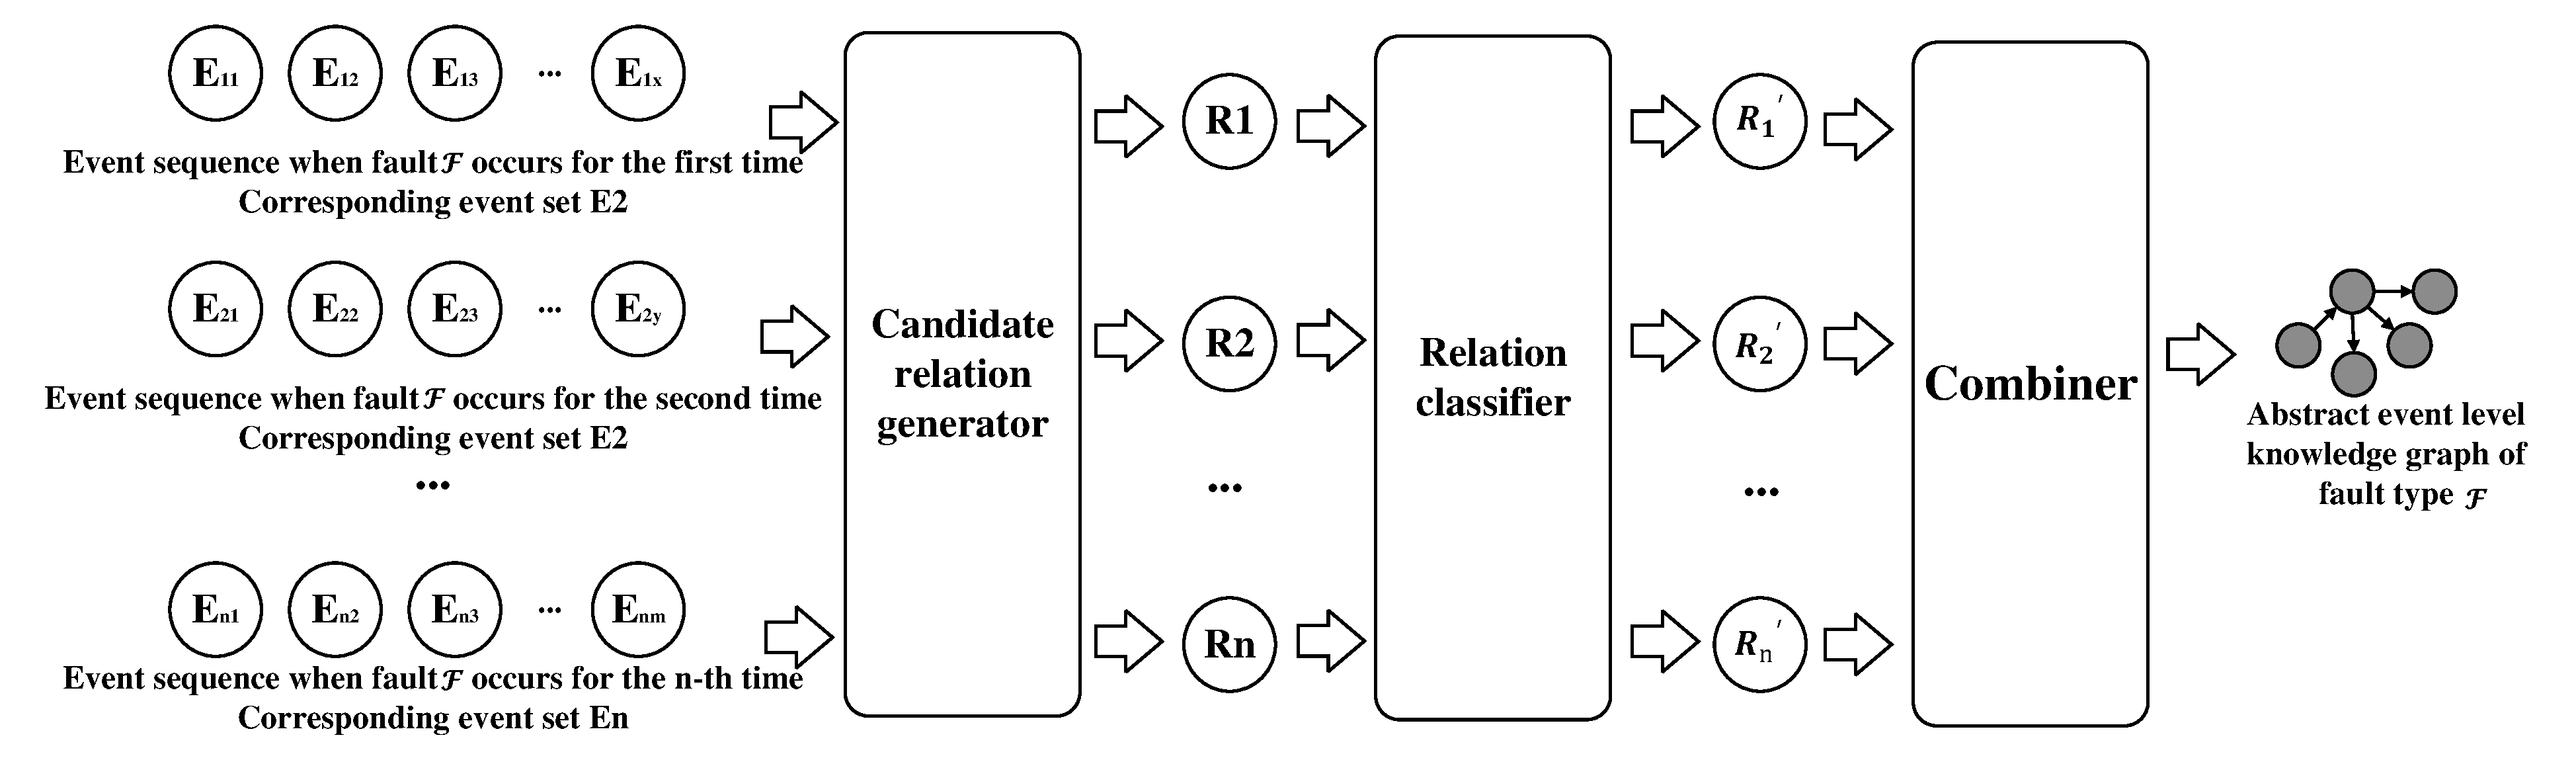
\includegraphics[width=.9\textwidth]{relation-combine.pdf}
    \caption{对应故障类型A的组件-事件知识图谱生成流程\label{relation-combine}}
\end{figure}

图\ref{relation-combine}是故障类型$\mathcal{F}$对应的抽象事件层知识图谱构建流程。下面是故障类型$\mathcal{F}$对应组件-事件知识图谱的具体构建步骤描述:
\begin{itemize}
    \item [(1)] 
    生成候选关系集合。获取故障类型$\mathcal{F}$发生$n$次$\mathcal{F}_1,\mathcal{F}_2,…,\mathcal{F}_n$分别对应时间段内的事件集合$E_1,E_2,…,E_n$。针对每个时间段内的事件集合,首先基于TFIDF\cite{joachims1996probabilistic}筛去部分白噪声事件后将事件按时间顺序前后相连,得到候选关系集合$R_1,R_2,…,R_n$。  
    \item [(2)]
    生成因果关系集合。对候选关系集合$R_1,R_2,…,R_n$分别使用训练好的关系分类器判别该集合中每条候选关系是否为因果关系,仅保留判别为“存在”的因果关系,得到对应关系集合${\mathbf{R}_\mathbf{1}}^\prime$、${\mathbf{R}_\mathbf{2}}^\prime$、…、${\mathbf{R}_\mathbf{n}}^\prime$。
    \item [(3)]
    规约生成抽象事件因果拓扑。对分类器保留后的关系集合${\mathbf{R}_\mathbf{1}}^\prime$、${\mathbf{R}_\mathbf{2}}^\prime$、…、${\mathbf{R}_\mathbf{n}}^\prime$取并集,融合$\mathcal{F}$故障类型各个时间段内的事件因果关系对,其中每个事件都会按照类型归约到抽象事件,从而获得$\mathcal{F}$故障的抽象事件因果关系集合$\mathcal{E}_{cause}=\ {\mathbf{R}_\mathbf{1}}^\prime\cup{\mathbf{R}_\mathbf{2}}^\prime\cup\ldots\cup{\mathbf{R}_\mathbf{n}}^\prime$。
    \item [(4)]
    规约生成组件层拓扑。由于在相同应用上触发的故障,其组件层有着相同的拓扑逻辑结构。只需要将每个故障时间段组件图整合起来即可,具体整合方式为把具体id去除,只保留组件类型。如位于两个时间段的“ts-voucher-mysql-75945d946-x6hwl”和“ts-voucher-mysql-5sdf45sdd-xz45z”可以归约到组件实体“ts-voucher-mysql”。此外,针对“ts-voucher-mysql-75945d946-x6hwl”上发生“22:08:57/1575900537 找不到票务信息”这种组件到事件的关系,在组件-事件知识图谱中该关系会被存为“ts-voucher-mysql”上发生“找不到票务信息”。最后为了区分负载“ts-train-service”的Container,和负载“ts-ticketinfo-service”的Container,本文选择如文献\parencite{qiu2020causality-mining-knowledge-graph}对同类型组件进行序号标注的方式,将上述两个Container分别标注为“container1”,“container2”。
    \item [(5)]
    生成故障类型$\mathcal{F}$对应的组件-事件知识图谱。融合生成的关系对集合$\mathcal{E}_{cause}$,得到对应的有向图即为故障类型$\mathcal{F}$对应的抽象事件层知识图谱。再将组件实体与抽象事件实体按产生关系进行连接,就可以得到故障类型$\mathcal{F}$对应的组件-事件知识图谱。
  \end{itemize}

\begin{figure}[htbp]
    \centering
    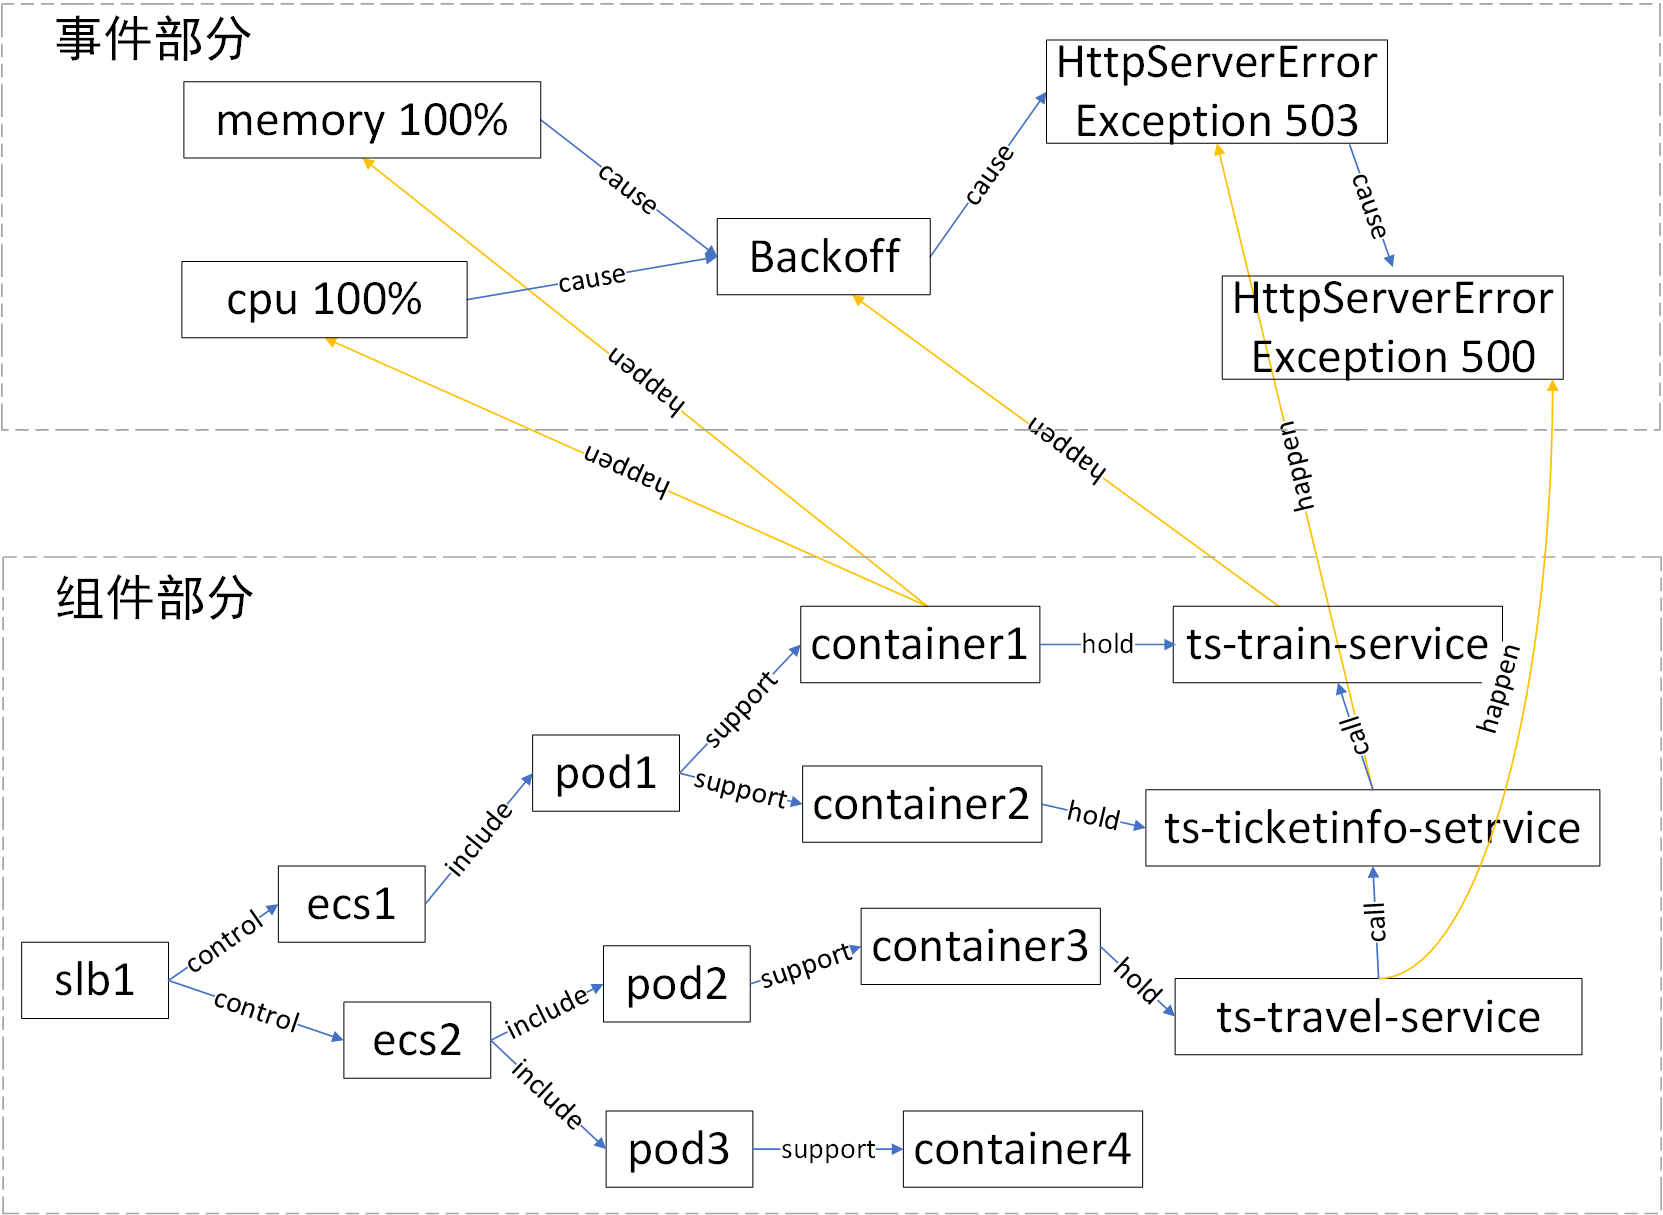
\includegraphics[width=.7\textwidth]{graph-example.png}
    \caption{数据库不可用无法查票故障对应知识图谱部分示例\label{graph-example}}
\end{figure}

图\ref{graph-example}是故障类型“数据库不可用无法查票”对应的组件-事件知识图谱的一部分。该知识图谱中,组件部分清晰地展示了ts-train-sevice,ts-ticketinfo-service,ts-travel-service分别部署在3个Container容器上,而这些容器托付在多个Pod中。同样的,这些Pod被负载在2台云服务器ECS中,并且这些ECS又被一台负载均衡器SLB所调控。在抽象事件部分,抽象事件实体被因果关系连接构成了抽象事件图,该图沉淀了ts-travel-service发生HttpServerError Exception 500故障的触发链知识。另外,抽象事件部分与组件部分被happen关系连接,本质上描述了抽象事件在哪类组件上产生。

\section{本章小结}
本章主要介绍了组件-事件知识图谱的构建方式。对于组件部分数据,云服务商会提供开放的API返回分布式集群含有的组件属性信息、组件数量及每个组件间的关联关系,微服务访问追踪系统可以获取微服务间访问拓扑关系。在事件数据层面,通过聚类、异常检测算法和模板匹配将多源异构数据统一为了事件类型数据,随后训练关系分类器挖掘事件间因果关系,最后将历史数据按照故障类型分组再沉淀生成对应故障类型的组件-事件知识图谱。下一章会在此基础上,研究组件-事件知识图谱的表示学习工作。

% 知识图谱可以用资源描述框架(RDF)\cite{heim2009relfinder}来表示,它包含一个主语、谓语和宾语,如等式\ref{rdf}所示。RDF由节点和边组成。节点表示实体和属性,边表示实体和实体之间的关系以及实体和属性之间的关系。
% \begin{equation}
%     Subject \stackrel{predicate}{\longrightarrow} Object
%     \label{rdf}
% \end{equation}

% 定义2:抽象事件。抽象事件是同类型事件规约后的形式。只包含包括3个部分:
% TypeId:抽象事件唯一标识;
% LocationType:抽象事件发生在何种组件上;
% Event type:抽象事件类型名;
% 定义3:事件知识图谱。事件知识图谱是三元组集合(抽象事件e_1,r,抽象事件e_2),其中r为因果关系。
